% ~ 6 pages
\chapter{The ATLAS Experiment at the Large Hadron Collider}
\label{chap:atlas}

\section{The Large Hadron Collider}
\label{sec:lhc}

\section{The ATLAS Experiment}
\label{sec:atlas}

\begin{figure}[ht]
  \centering
  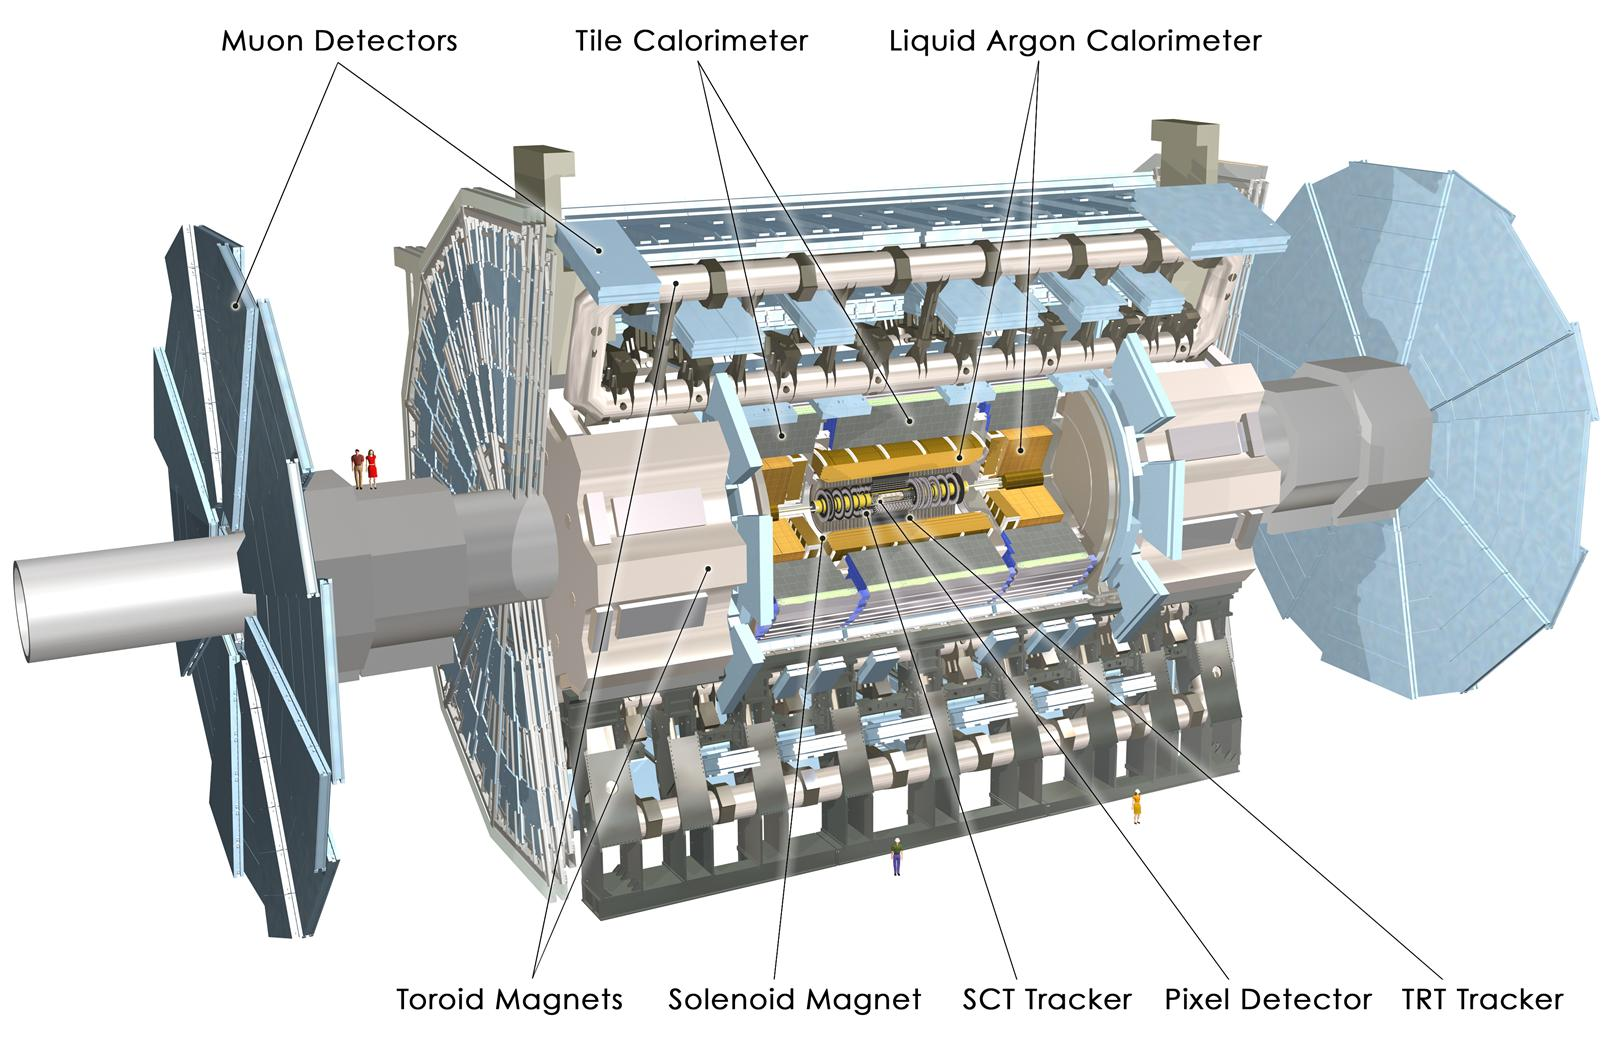
\includegraphics[width=0.8\textwidth]{./figures/atlas/overview.jpg}
  \caption{Overview of the ATLAS detector\cite{atlas_detector}}
  \label{fig:atlas_indet}
\end{figure}

\cite{atlas_detector}

\subsection{Coordinate System}
\label{sec:atlas_coord_sys}

ATLAS right-handed coordinate system. Origin at IP, z-axis in beam direction.
x-axis points to the centre of the ring. y-axis points upwards. $x$,$y$ span the
transverse plane. Cylindrical coordinates can be used $(r, \phi, z)$ with the
azimuthal angle $\phi$. Or spherical coordinates $(r, \phi, \theta)$ with the
polar angle $\theta$ with respect to the beam direction $z$ is used.

Momentum conservation only in transverse plane due to unknown momentum in
longitudinal direction leads to the 'definition' of $p_\text{T}$. Rapidity $y$
and pseudorapidity $\eta$ differences Lorentz-invariant (only boost along the
$z$-axis) in the massless limit.

\begin{align*}
  p_\text{T} &= | \vec{p} | \, \cos\theta \\
  y &= \frac{1}{2} \ln\frac{E + p_z}{E - p_z} \\
  \eta &= -\ln\tan\left( \frac{\theta}{2} \right) \\
  \Delta R &= \sqrt{(\Delta\eta)^2 + (\Delta\phi)^2}
\end{align*}

\begin{itemize}
\item $\Delta R$: Lorentz-invariant in the massless particle limit (otherwise
  the same definition but with rapidity instead of pseudorapidity is required)
\item Transverse energy $E_\text{T}$
\item Missing transverse energy $E_\text{T}^\text{miss}$
\end{itemize}

\subsection{Tracking System}
\label{sec:atlas_tracking}

\begin{figure}[ht]
  \centering
  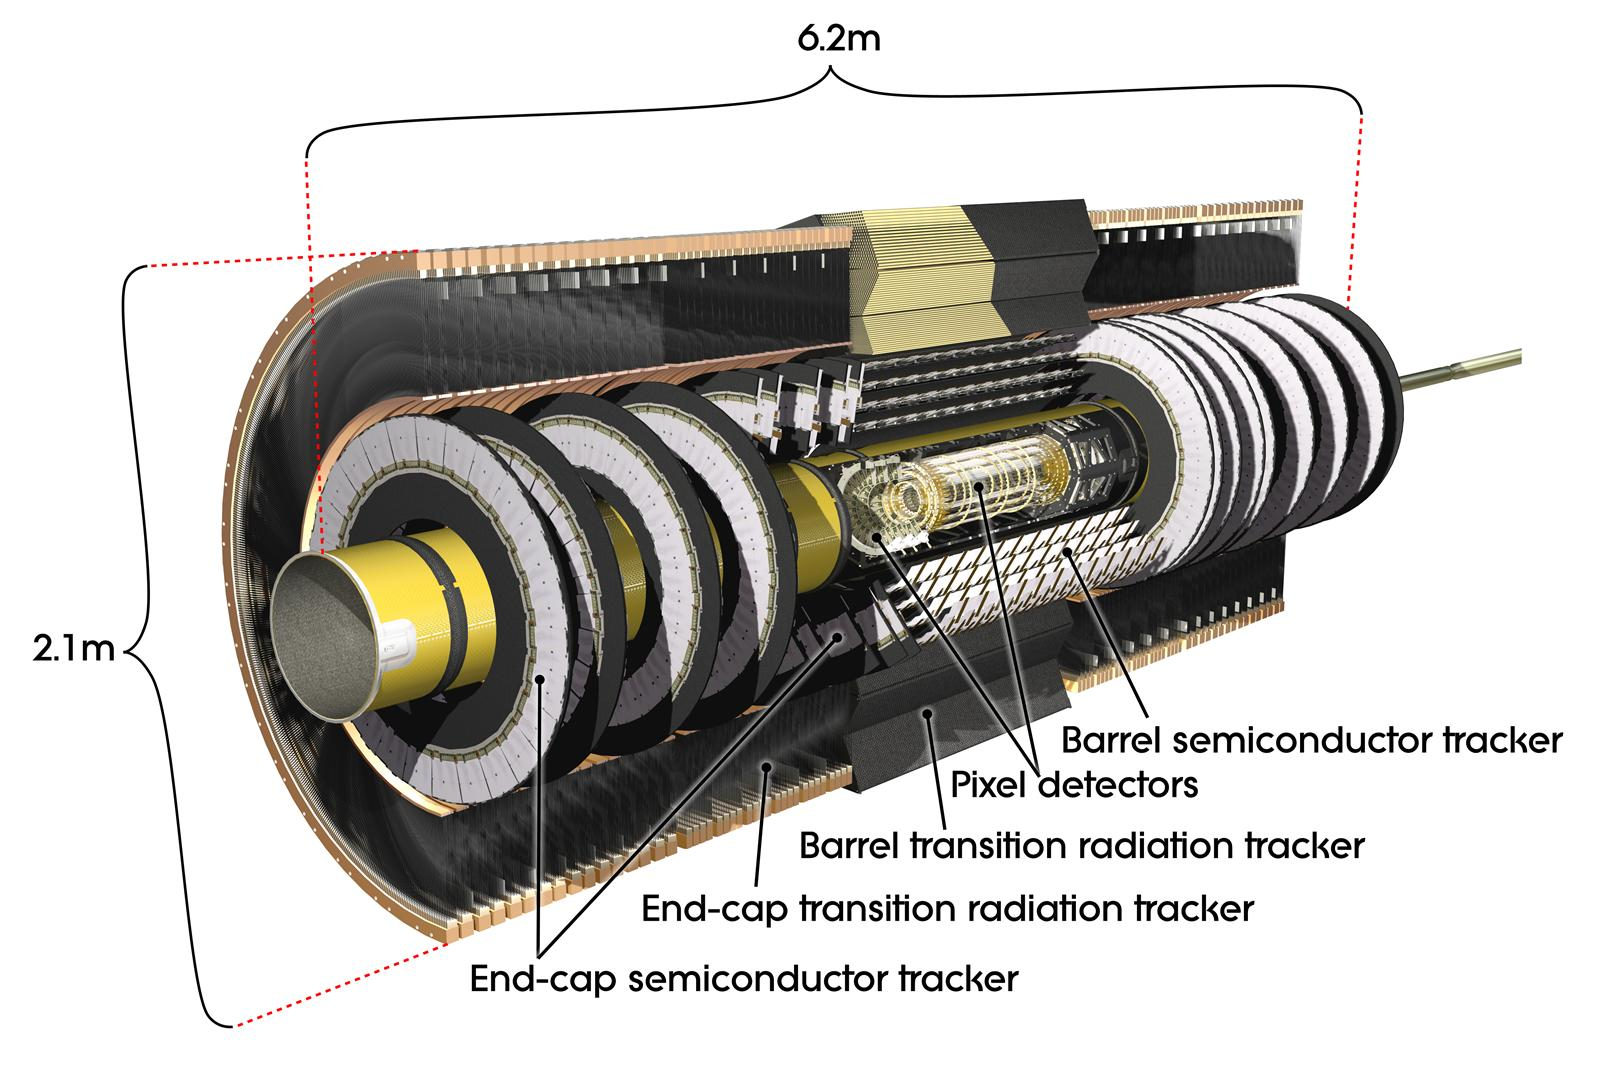
\includegraphics[width=0.75\textwidth]{./figures/atlas/inner_detector.jpg}
  \caption{ATLAS inner detector\cite{indet_fig} also in \cite{atlas_detector}}
  \label{fig:atlas_indet}
\end{figure}

\todo[inline]{Name this 'Inner Detector'?}
\todo[inline]{Introduce abbrev.\ ID}
\todo[inline]{Introduce abbrev.\ IBL}
\todo[inline]{Define impact parameter: $d_0$ and $z_0$.}
\todo[inline]{Define perigee}
% See \url{https://twiki.cern.ch/twiki/bin/view/AtlasProtected/InDetTrackingDC14#Impact_parameters_z0_d0_definiti}

\todo[inline]{Find primary sources on this stuff!}
\begin{itemize}
\item Track \& vertex reconstruction
\item Charged particles provide hits in ID
\item High spacial resolution to reconstruct tracks in dense environments
  (number of tracks per event -- 200? -- check this)
\item Solenoid field with \SI{2}{\tesla}
\item Secondary vertex reconstruction (B-layer -- this is important, Pixel, SCT)
\item TRT -- 'continuous' tracking (what is this?) and distinction between
  electrons and hadrons using transition-radiation
\item ID acceptance $|\eta| < \num{2.5}$
\item Split into barrel and two endcap regions
\item Pixel: Three barrel layers, three endcap layers each (and 1 layer IBL).
  Pixel detector in 'Pixel Support Tube' to allow exchange of elements in case
  of radiation damage. Inner Radius \SI{4.2}{\centi\metre} and outer radius
  \SI{25}{\centi\metre}.
\item The layer after the IBL is called B-layer!
\item IBL \cite{ibl_tdr}: Improve B-tagging when modules in the remaining pixel layers fail;
  Tracking inefficiencies at high pileup affects B-layer needs redundancy;
  Better impact parameter reconstruction improves vertexing and b-tagging
\item Pixel layers segmented in $r\varphi$ and $z$. Single pixel
  \SI{50}{\micro\metre} in $r\varphi$ and \SI{400}{\micro\metre} in $z$
\item Silicon strip detectors (four layers) in support structure with radius of
  about \SI{55}{\centi\metre}
\item SCT strip detectors \SI{15}{\micro\metre} $r\varphi$ and
  \SI{70}{\micro\metre} $z$ resolution
\item TRT: Barrel region $|\eta| < \num{0.5}$, on average a track causes 36
  hits; Resolution decreases with pile-up
\end{itemize}

\subsection{Calorimeter System}
\label{sec:atlas_calo}

\todo[inline]{Topoclustering}
\todo[inline]{EM and LC scale}
\todo[inline]{Introduce nomenclature: strip layer, EM1, EM2, EM3, HAD}


\begin{figure}[ht]
  \centering
  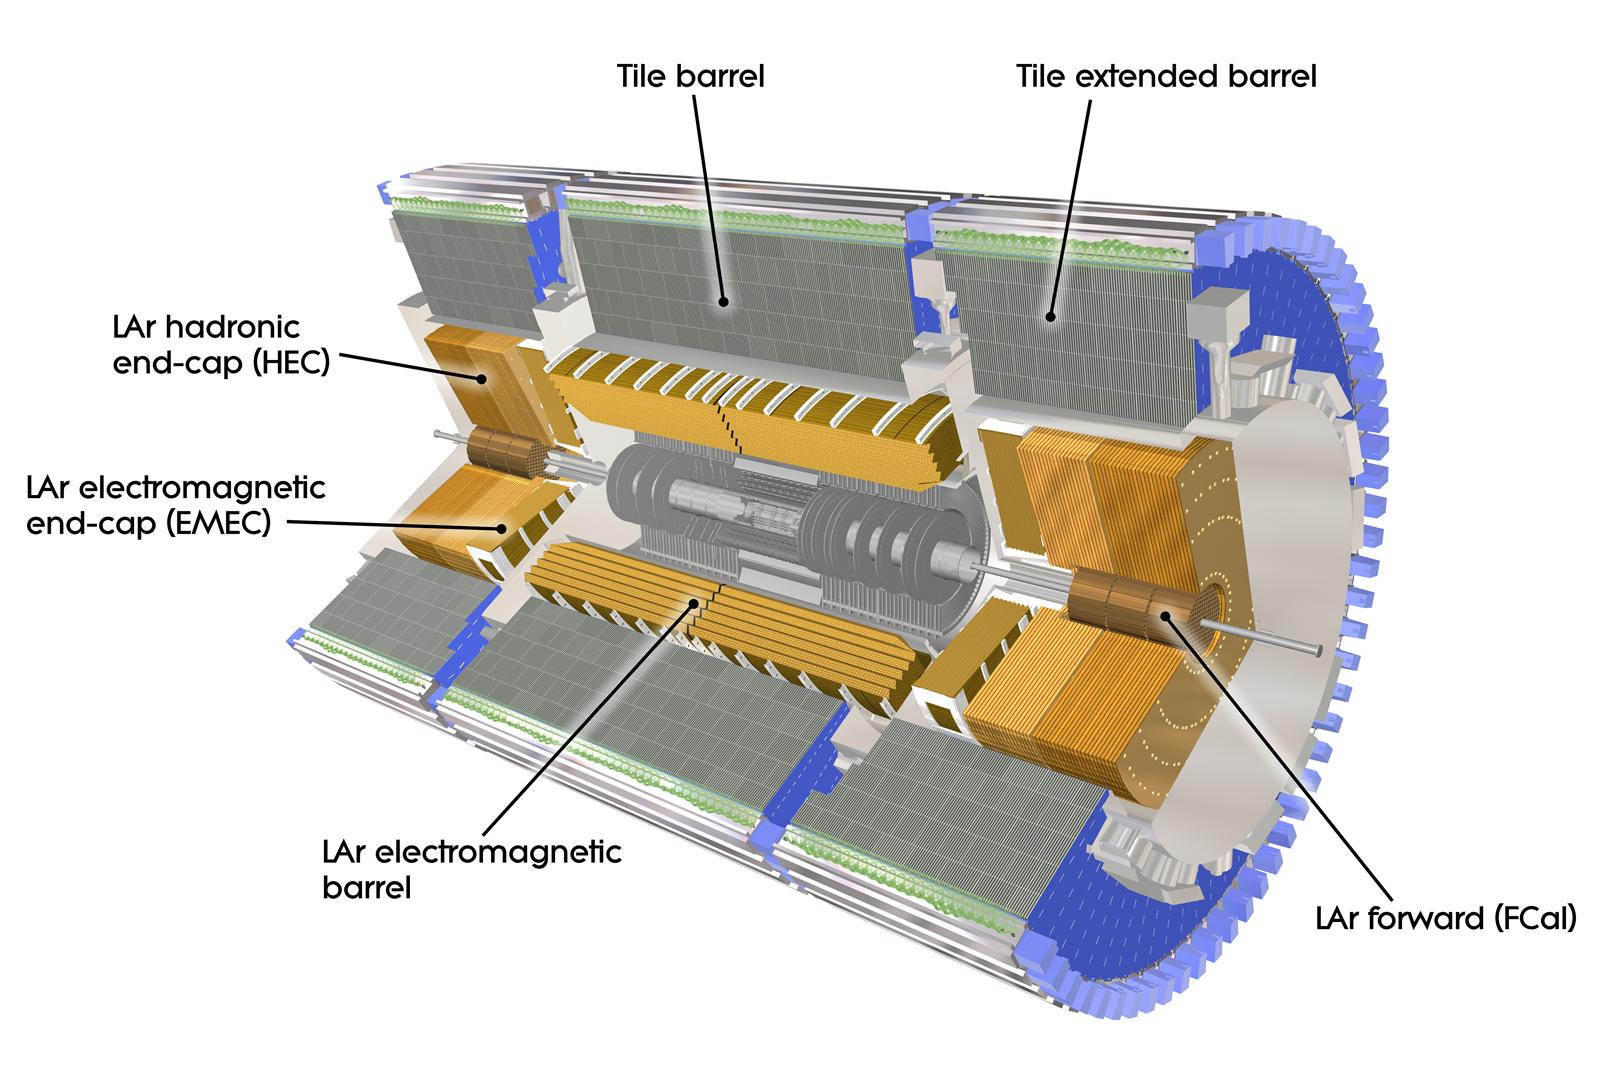
\includegraphics[width=0.8\textwidth]{./figures/atlas/calorimeter.jpg}
  \caption{ATLAS calorimeter\cite{calo_fig} also in \cite{atlas_detector}}
  \label{fig:atlas_indet}
\end{figure}



\begin{itemize}
\item LHC (brief)

\item ATLAS
  \begin{itemize}
  \item Overview (Design goals) \\
    brief: Beam Line, Inner Detector \& Solenoid, Calorimeter, Muon System \&
    Toroid, Trigger

  \item Nomenclature (Coordinate system, Pseudorapidity, $\Delta R$,
    $p_\mathrm{T}$)

  \item Inner detector / Tracker (and why they are important for taus)
    \begin{itemize}
    \item Pixel, IBL
    \item SCT
    \item TRT
    \item  Transverse Momentum Resolution, Vertex \& Secondary Vertex
      reconstruction, Impact Parameter Resolution, $\eta$-Coverage
    \end{itemize}

  \item Calorimeter (and why they are important for taus)
    \begin{itemize}
    \item Presampler, LAr (EM1 - EM3), Had (Tile, LAr)
    \item Cell sizes, $\eta$-Coverage, Thickness $X_0$ / $\lambda$,
      Energy Resolution vs. $E$
    \item Topoclusters \& Cluster moments
    \end{itemize}

  \end{itemize}
\end{itemize}

%%% Local Variables:
%%% mode: latex
%%% TeX-master: "mythesis"
%%% End:
